\newcommand{\nomedoc}{User's Guide}
\newcommand{\versione}{1.0}
\newcommand{\versioneglossario}{4.0}
\newcommand{\versionenormeprogetto}{4.0}
\newcommand{\nomefile}{User's Guide-\versione.pdf}
\newcommand{\datacreazione}{24 February 2011}
\newcommand{\datamodifica}{19 March 2011}
\newcommand{\stato}{formal}
\newcommand{\uso}{external}
\newcommand{\redazione}{Caputo Cosimo, Mandolo Andrea }
\newcommand{\verifica}{Palazzin Alberto}
\newcommand{\approvazione}{Trezzi Giovanni}
\newcommand{\distribuzione}{
VT.G \\
& Prof. Vardanega Tullio\\
& Prof. Cardin Riccardo }

% FUNZIONI TIPOGRAFICHE
\newcommand{\co}{\texttt} % courier
\newcommand{\bo}{\textbf} % bold
\newcommand{\pr}{\par\medskip} % paragrafo spaziato
\newcommand{\sca}{\textsc} % small caps

\documentclass[a4paper,12pt]{report}
% 10pt,11pt,12pt
% titlepage, notitlepage -> per dare inizio o no ad una nuova pagina dopo titolo
% twoside -> per dire se fronte-retro
\usepackage[latin1]{inputenc}
% per caratteri accentati
\usepackage[italian]{babel}
% per regole sintattiche italiane
\usepackage[bookmarks=true, pdfborder={0 0 0 0}]{hyperref}
% per collegamenti ipertestuali
\usepackage{graphicx}
% per inserimento immagini

% \usepackage{enumerate}
% per personalizzare elenchi puntati

\usepackage[hmargin=2cm]{geometry} %margine 2 cm
%\geometry{options varie}

% comandi per gestire meglio header e footer
\usepackage{fancyhdr}  % header e footer
\usepackage{totpages}
\pagestyle{fancy}
\renewcommand{\headrulewidth}{0.4pt}
\renewcommand{\footrulewidth}{0.4pt}

\setlength{\headheight}{1.2cm} % NON TOCCARE
\setlength{\voffset}{-1.5cm} % NON TOCCARE
\setlength{\textheight}{666pt} % NON TOCCARE
\setlength{\footskip}{60pt}
\setlength{\parindent}{0pt} % INDENTAZIONE

\lhead{\nomedoc\  (ver. \versione)}
\chead{}
\rhead{
\includegraphics[height=1cm]{img/netmus.png}}
\lfoot{
\includegraphics[height=0.8cm]{img/logo.png}}
\cfoot{}
\rfoot{\thepage}

\usepackage{titlesec}
\titleformat{\chapter}{\normalfont\huge\bfseries}
{\thechapter}{20pt}{\Huge}

\usepackage{rotating}   % PER TABELLE E AMBIENTI RUOTATI
\usepackage{array}
\usepackage{color}
\usepackage{colortbl}  % VARIE PER GESTIRE I COLORI
\definecolor{Orange}{RGB}{255,127,0}   % ARANCIO ACCES0
\definecolor{orange}{RGB}{255,207,80}  % ARANCIO TENUE

\addtocontents{toc}{\protect\thispagestyle{fancy}}  % PER INDICI CON + PAGINE
\usepackage[font=it]{caption}    % PER RENDERE CORSIVE LE DIDASCALIE
\usepackage{eurosym}  % PER SIMBOLO EURO

% \usepackage{listings}   per codice sorgente

\author{VT.G - Valter Texas Group}

\begin{document}

\pagenumbering{Roman} % INIZIO NUMERAZIONE ARABA

\vspace*{1cm}
\begin{center}


\includegraphics[width=9cm]{img/logo.png}\\
\vspace{0.5cm}
\begin{LARGE} \sca{VT.G - Valter Texas Group} \end{LARGE}\\
\vspace{0.5cm}
\begin{Large}
\emph{valtertexasgroup@googlegroups.com} \end{Large}\\
\vspace*{1cm} 
\includegraphics[width=5cm]{img/netmus.png}\\
\vspace{0.5cm}
\begin{Large} \sca{\nomedoc} \end{Large}\\
\vspace{1cm}
\begin{Large} \emph{Software Engineering A.A. 2010-2011} \end{Large}\\
\end{center}
\vspace{1cm}

% INFORMAZIONI DOCUMENTO
\begin{center}
\begin{tabular}{r|l}
\hline & \\
\bo{Name} & \nomefile \\
\bo{Current Version} & \versione \\
\bo{Creation} & \datacreazione \\
\bo{Last Modify} & \datamodifica \\
\bo{State} & \stato \\
\bo{Use} & \uso \\
\bo{Editing} & \redazione \\
\bo{Control} & \verifica \\
\bo{Approbation} & \approvazione \\
\bo{Distribution} & \distribuzione \\
& \\\hline
\end{tabular}
\end{center}
\newpage

\chapter*{Summary}
\thispagestyle{fancy}
This document is a simply and intuitive guide for beginners using NetMus
system.\\
It includes a glossary where you can find more-difficult terms that are used
here and an appendix with the most common problems that you can encounter,
possible reasons that caused the problem and possible solutions. 

\newpage
% REGISTRO MODIFICHE
\section*{Change log}

\begin{longtable}{|p{0.13\textwidth}|c|p{0.2\textwidth}|p{0.46\textwidth}|}
\hline
\rowcolor{orange} \bo{Date} & \bo{Version} & \bo{Author} & \bo{Description} \\
\hline
\endhead
\hline
\endfoot
19/03/2011 & 1.0 & Trezzi Giovanni & Document validation.\\
\hline
18/03/2011 & 0.6 & Palazzin Alberto & Document verified.\\
\hline
17/03/2011 & 0.5 & Caputo Cosimo & Translation finished.\\
\hline
17/03/2011 & 0.4 & Caputo Cosimo & Updated screenshots.\\
\hline
14/03/2011 & 0.3 & Mandolo Andrea & Some grammatical corrections.\\
\hline
10/03/2011 & 0.2 & Mandolo Andrea & Partial translation finished.\\
\hline
28/02/2011 & 0.1 & Caputo Cosimo & Starting the translation.\\
\end{longtable}

% INDEX
\tableofcontents

\chapter{Introduction}
\thispagestyle{fancy} % serve perche' nelle pagine di inizio Chapter esca header e footer
\pagenumbering{arabic} % INIZIO NUMERAZIONE NORMALE
\rfoot{\thepage\ of \pageref{TotPages}}
This guide was created for beginners that want start using \co{NetMus}, and it
includes a description of the product and the instructions for use it. There are
also two appendix in where you can find most common error messages and a
glossary.\\

All the terms in the glossary are underlined in the document in their first
occurrence \underline{like this}.

\section{Description of the Product's User}
\co{NetMus} can be used by everyone: you need to know only the basics like using
a \underline{web browser} and navigating through internet. 


\section{How to Read this Guide}
This Guide presents the product \co{NetMus} and describes its functionality and
also the user's approach using the system. In particular it will show the 
actions that you can perform with the software and how to resolve, if it is
possible, problems that you can encounter using it.

\section{How to report problems and errors}
If you found any problems you can report it with the online service provided by
Google at this link:  \url{http://code.google.com/p/netmus/issues/list}.\\
You just have to click on top-left button \emph{New issue} (figure
\ref{fig:issues}), and fill the module's
fields (figure \ref{fig:newIssue}) with a name (2) for the problem and a short description of it (3). 

\begin{figure}[!htbp]
  \centering
  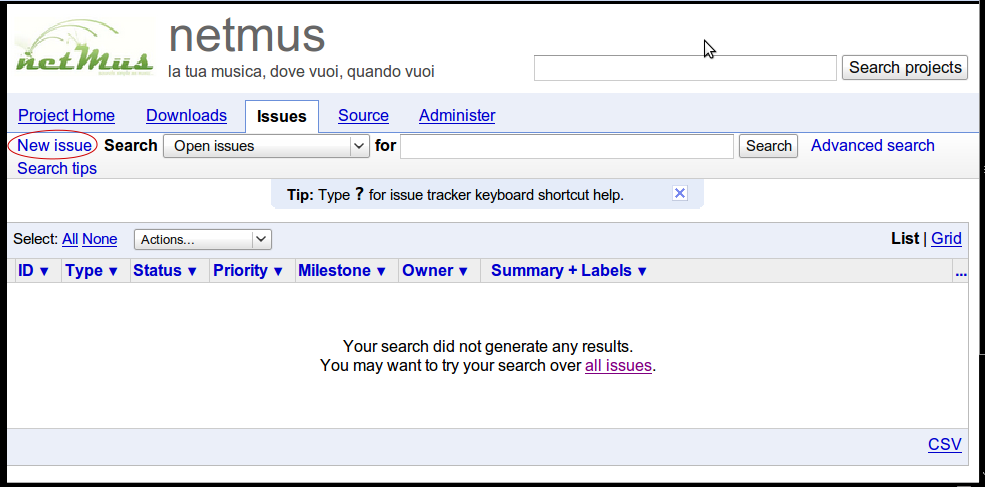
\includegraphics[width=16cm]{img/MU/issues.png}
\caption{Opening a new issue}
\label{fig:issues}
\end{figure}

\begin{figure}[!htbp]
  \centering
  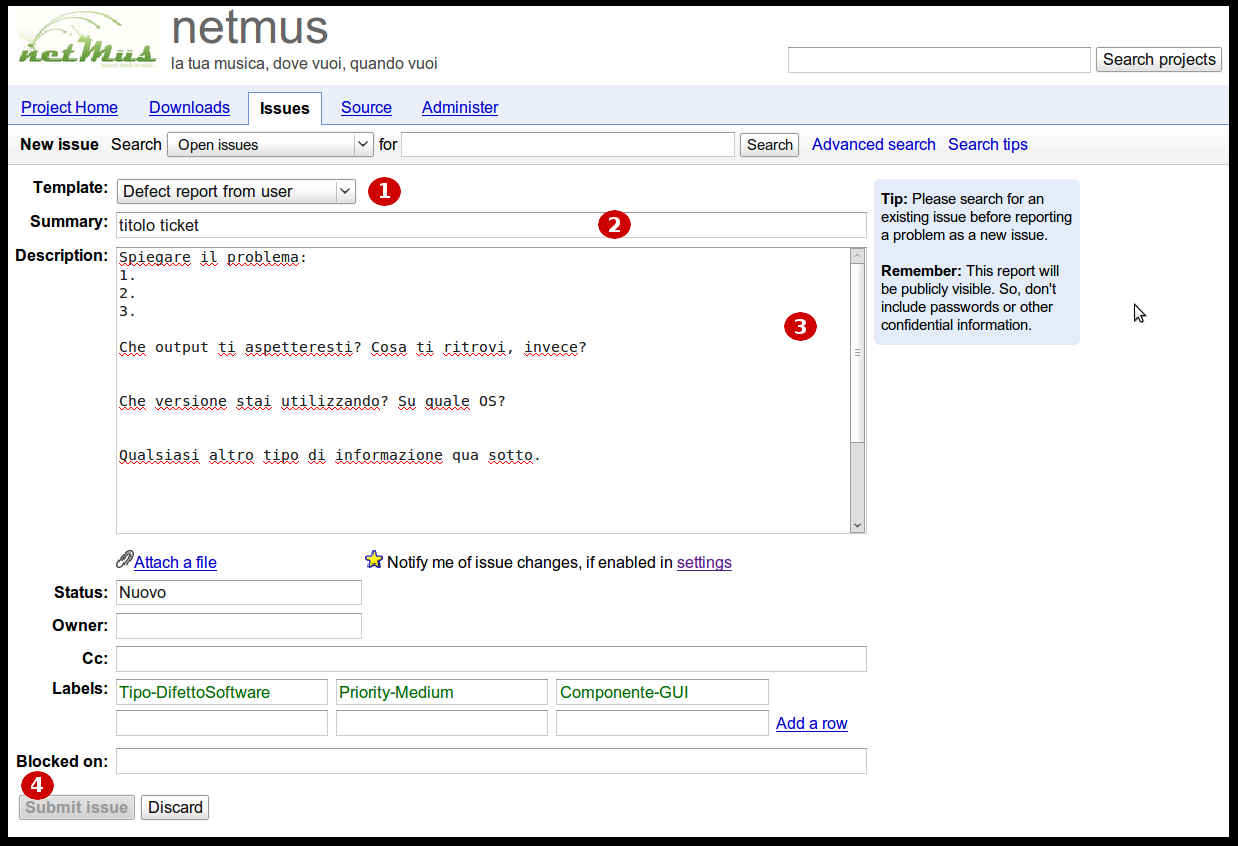
\includegraphics[width=16cm]{img/MU/new_issue.png}
\caption{New issue module}
\label{fig:newIssue}
\end{figure}

If you want an help to describe the problem, you can use the template
\emph{Defect report from user} (1) that contains a track that will help you writing all 
informations needed.\\

Once you have compiled it, press the ``Submit issue'' button (4).

\section{Informational references}
In case of further clarification on used , or for further
help, you can refer to: \url{http://docs.google.com/support/
} .

\chapter{General Description}
\thispagestyle{fancy}
Today, the biggest part of the population listen their music in digital
format: it's for that reasons that was introduced \co{NetMus}, an useful
application that allows sharing our preferred music and listening it on online
streaming, and that was created with modern technologies like \underline{cloud
computing}.\\

\co{NetMus} allows users to have a virtual online library with all their
preferred songs, and to listen this songs everywhere.\\

Using the product is very simple. Just after you get logged to \co{NetMus} you
only have to connect your Mp3 player with the pc and the system will start
working automatically. Otherwise you can also scan a local directory of your PC
that contains music in the mp3 format: all the songs will be fully extracted,
analysed and inserted in your profile on your \co{NetMus} account, ready to be
listened.\\

Between \co{NetMus}' functionalities we have streaming youtube player for audio
and video broadcasting, possibility to create your own playlists, and many other
utilities.\\

All the system is decorated with a simple and intuitive graphical interface
with the complete access to all the necessary functionalities.\\

\chapter{Using Instructions}
\thispagestyle{fancy}

\section{Functional Description}
In this chapter we show a complete guide for \co{NetMus} use.\\
You will find a section were are listed all the requirements for a well
working approach with \co{NetMus}, then you will encounter a detailed overview
with the description of all the actions you can perform with the
application.

\subsection{Recommended System Requirements for NetMus Use}
\co{NetMus} is a web application that is viewed and used with your web browser.
Although you reached it by internet navigation, you don't need only an internet
connection and a web browser to use it.\\

Now we show a list of the requirements for using \co{NetMus}.

\begin{itemize}
  \item Internet Connection (higher than 56k)
  \item Web Browser (Google Chrome, Safari, Opera, Firefox*, IE**)
  \item A JVM (Java Virtual Machine) correctly installed on your PC
  \item Adobe Flash Player plugin for video broadcasting
  \item Javascript activated on your web browser
\end{itemize}

Without anyone of this tools you will not able to use
correctly all the system functionalities, or even you will unable to use
it at all.\\
\\
\\

\emph{* If you use Firefox, you won't see the animation effects of the
system, because Firefox doesn't support animations.}\\ 
\emph{** If you wanna use NetMus with Microsoft Internet Explorer, you have to
download the Google Chrome Frame plugin for IE, because this web browser doesn't
support the advanced functionalities of NetMus: you will be prompted by its
setup the first time you open NetMus}\\

\newpage
\section{Using NetMus}
Let's look at how to use \co{NetMus}

\subsection{Registering to NetMus}

Go at the link \url{http://netmusbeta.appspot.com} to start using \co{NetMus}.\\
\begin{figure}[!htbp]
  \centering
  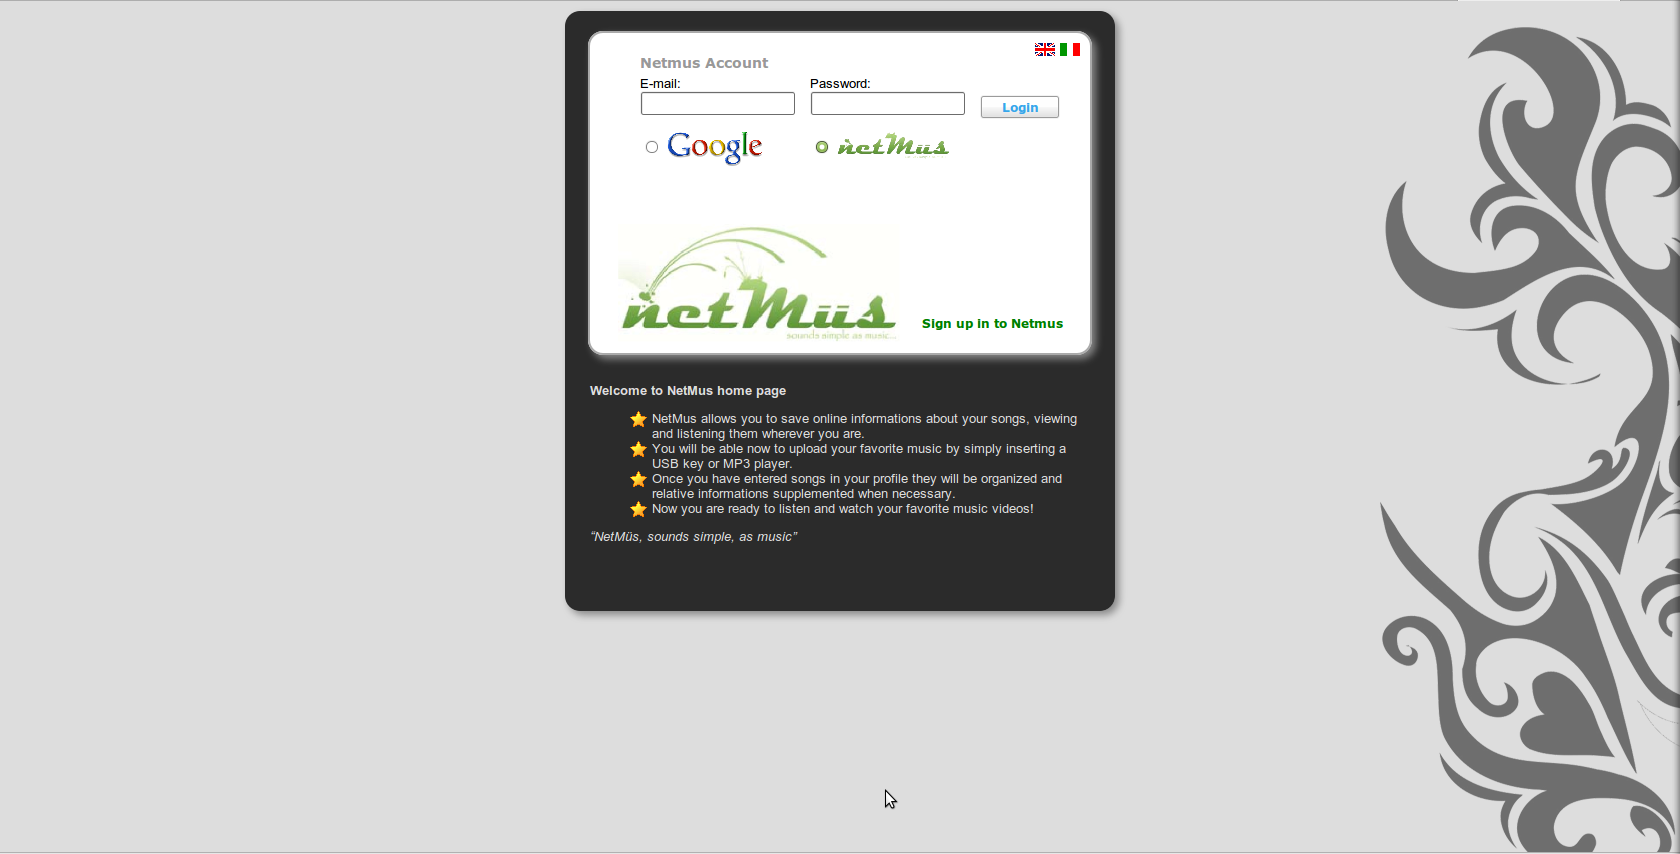
\includegraphics[width=14cm]{img/MU/login.png}
\caption{Interface of NetMus login}
\label{fig:login}
\end{figure}
\\
Here is the login page to enter \co{NetMus} (figure \ref{fig:login}). If you are
a Google user, you can join \co{NetMus} using your Google account, or create a
new account on the system.

\subsubsection*{Login using a Google account}
You have to select the Google login and click on the button ``Log in
NetMus using your Google Account'' (figure \ref{fig:loginGoogle}). You will be
redirected to the Google login page, here you get logged in and then you will be redirected again to
\co{NetMus}, but this time you will be logged to the system.\\

\begin{figure}[!htbp]
  \centering
  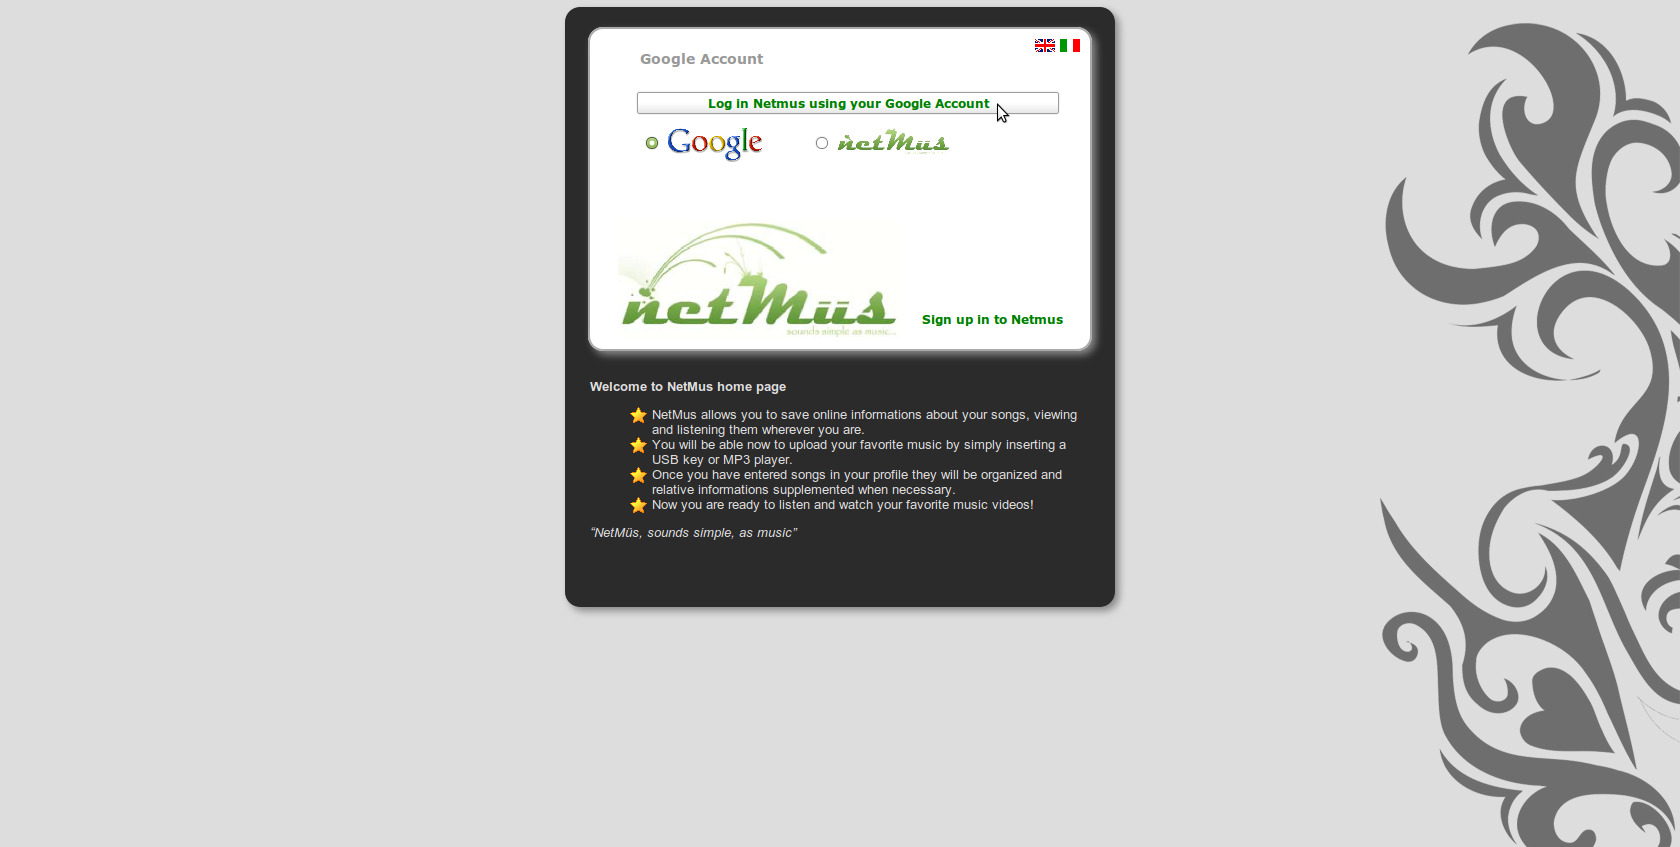
\includegraphics[width=14cm]{img/MU/loginGoogle.png}
\caption{Interface to Google login}
\label{fig:loginGoogle}
\end{figure}

\subsubsection*{Creating a new NetMus account}
If you aren't a Google user and this is your first access to \co{NetMus}, you
have to create your own account registering to the system.
\co{NetMus} registration and use are completely free.

To view the registration forms, just select the voice ``Sign up in to NetMus'',
and the view will change showing you registration fields (figure
\ref{fig:registrazione}).

\begin{figure}[!htbp]
  \centering
  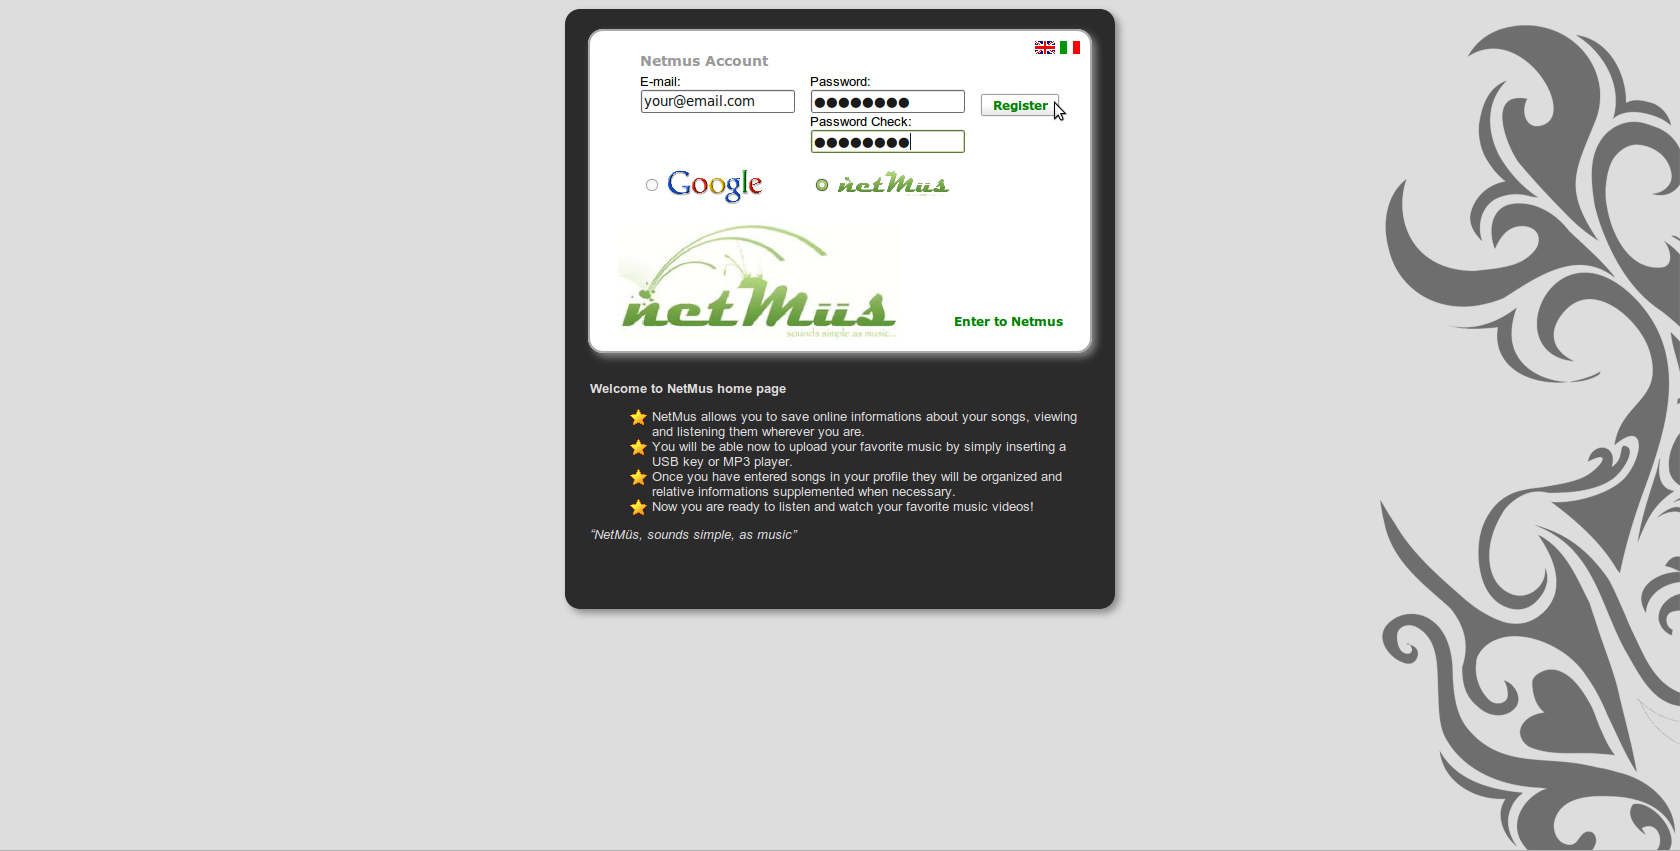
\includegraphics[width=14cm]{img/MU/registration.png}
\caption{Interface to join NetMus}
\label{fig:registrazione}
\end{figure}

To register yourself to the system you need to insert a correct email address
and a password with more than 5 characters. Once you have created your account,
you will have free access to \co{NetMus} system.

\newpage
\subsection{First Access to NetMus}

When you first access the system, on loading you
will be asked whether to run the signed applet, giving him permission to access
to your computer (figure \ref{fig:permessiApplet}).
\begin{figure}[!htbp]
  \centering
  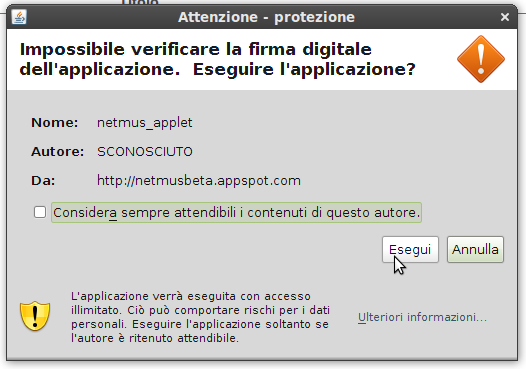
\includegraphics[width=10cm]{img/MU/permessi_applet.png}
\caption{Execution request of the applet}
\label{fig:permessiApplet}
\end{figure}

The applet is the \co{NetMus} component that seeks mp3's on your computer and
extract datas: \emph{it does not collect other information about you, and do not
contain any viruses}.

If you deny permission, the applet wont be able to access the contents of your
computer and peripherals, thus preventing the collection of information
(and then you'll not be able to add tracks).\\
This dialog will appear to request authorization each
access, unless you select ``Always trust content of
this author'' before clicking on ``Run''.\\

The interface will be presented will be structured
in this way (figure \ref{fig:paginaPrincipale}): \ \

\begin{figure}[!htbp]
  \centering
  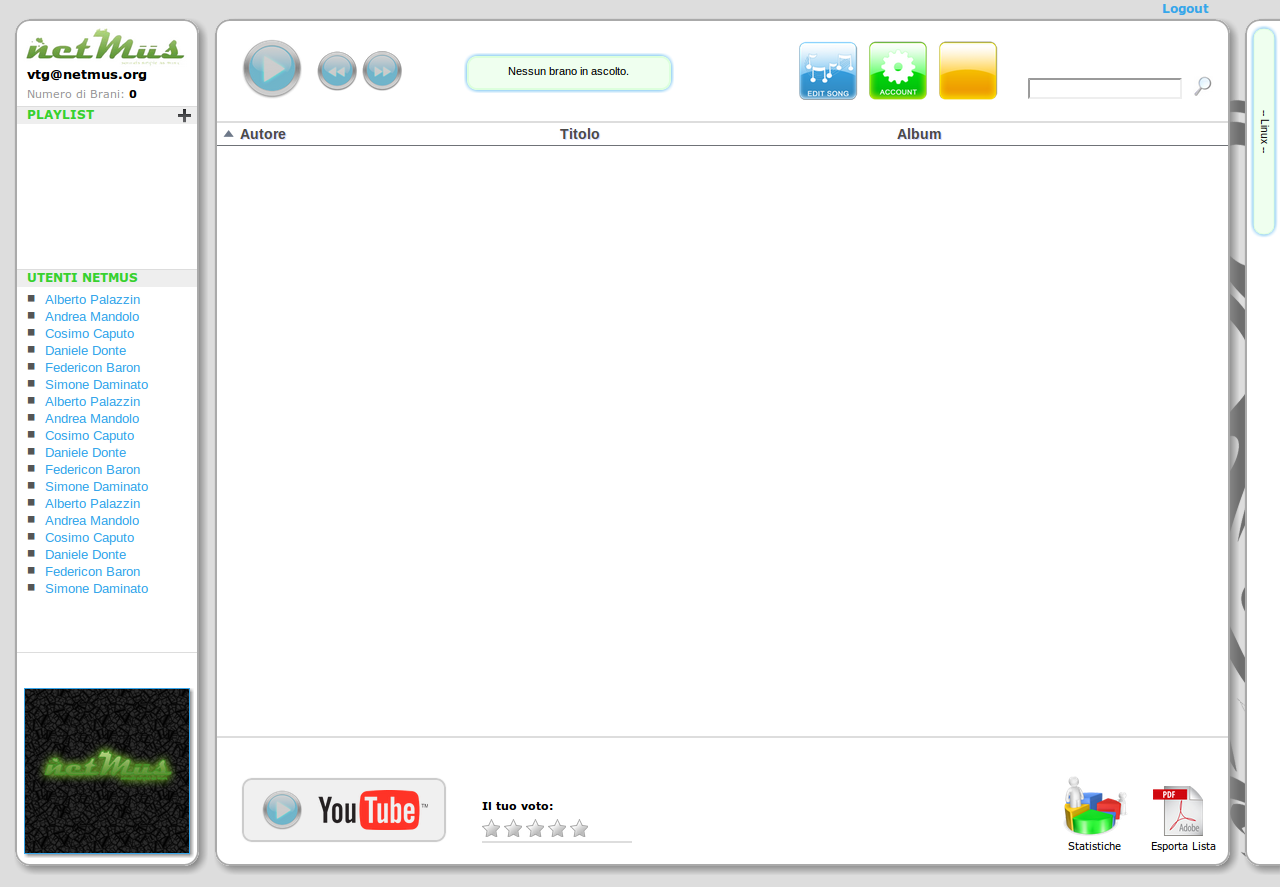
\includegraphics[width=15cm]{img/MU/profile_blank.png}
\caption{NetMus homepage at first access}
\label{fig:paginaPrincipale}
\end{figure}

There are three main parts: on the left we'll find the section of
playlists (1), in the middle the one of the tracks (2), and finally on the right
there is the section of the applet (the device scanner bar) (3).\\

Let's take a closer look (figure \ref{fig:appletbarAperta}):\\
\begin{figure}[!htbp]
  \centering
  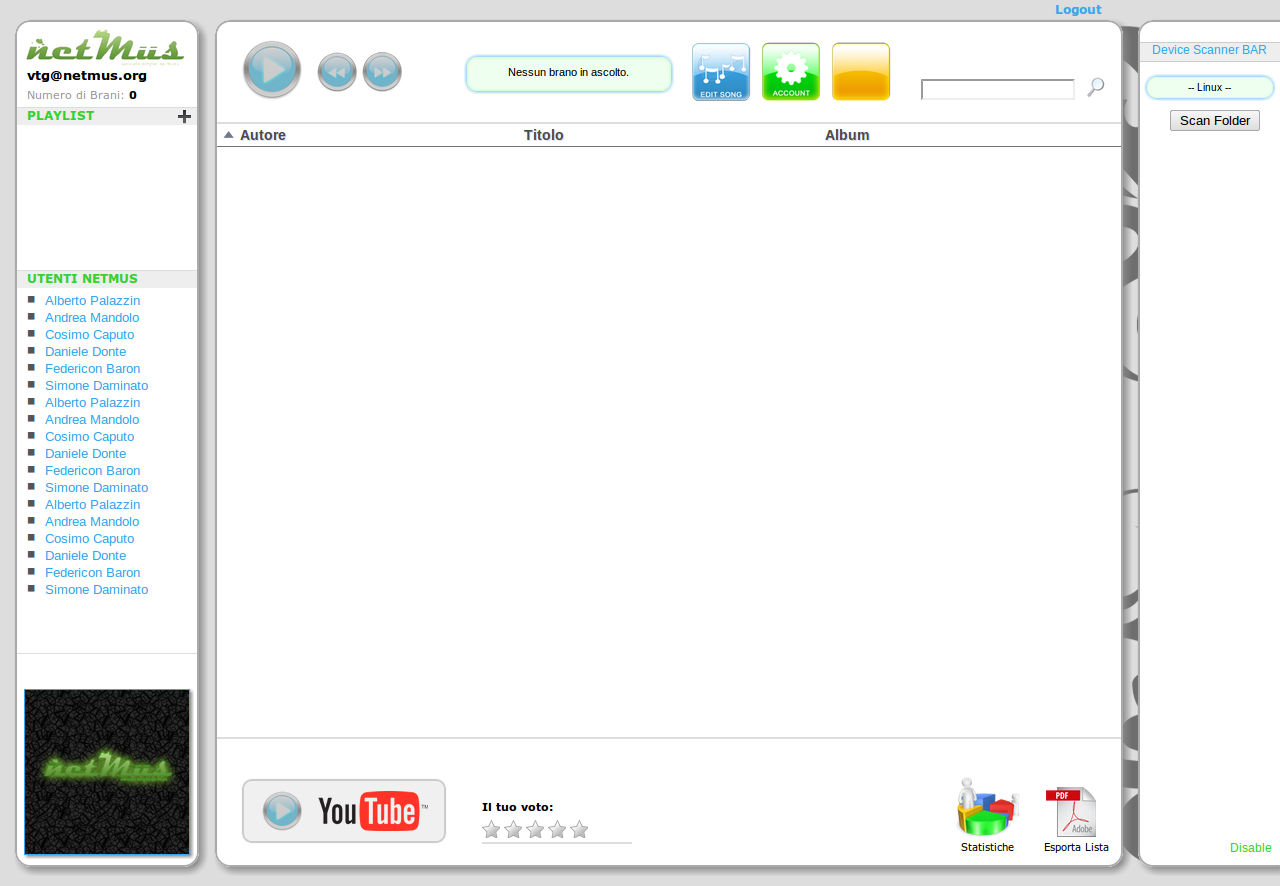
\includegraphics[width=14cm]{img/MU/applet_bar_open.png}
\caption{NetMus homepage with the DEVICE SCANNER BAR open}
\label{fig:appletbarAperta}
\end{figure} 

On the left menu, on the top (1) we find the \co{NetMus} logo and
your \underline{nickname}, that for now is your email address. It also presents
the number of songs contained in your songs' list, that are zero at your first
access. Under this (2), we can find the playlist menu (empty for the moment),
where you will find all the playlist created.\\

The central section is the most important part of the application, infact this
is our music library with control buttons (3), the searching form (4) (look at
\ref{cap:ricerca}), just below the songs' list (5) and on the bottom the
YouTube player (6).\\

At the right side of the page there is a bar called ``DEVICE SCANNER BAR'' that
allows the scanning process of the \underline{mass storage devices} (7). If you
hover this bar with your mouse pointer, the bar will expand: you can lock it in
this position by clicking on the padlock symbol (8).\\
The bar allows you to manually scan your pc and displays the progress of the
analysis and automatic or manual extraction of mp3 files from one device or from
the selected \underline{directory}.\\
You can also enable or disable the automatic scan by clicking on the text in the
lower right (9): when green indicates that the
automatic scanning is enabled, when it is red instead indicates that it's
off.

\newpage
\subsection{Start using NetMus}

First of all if you want to take advantage of the main \co{NetMus}' peculiarity,
the online music library, it is necessary to load some songs.\\
To do this, you can insert a mass storage device
into the USB port of your PC, otherwise it is possible to scan a directory of
your own PC, clicking on the ``Scan Folder'' button, then select the right
folder and press ``OK'' (figure \ref{fig:scansioneManuale}).\\

\begin{figure}[!htbp]
  \centering
  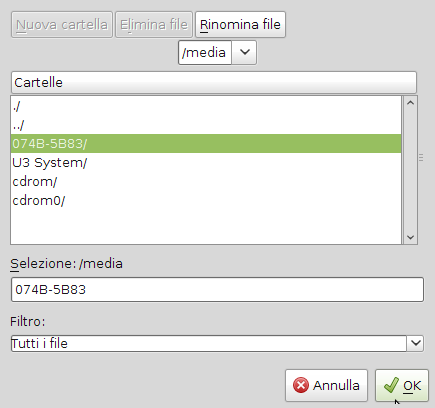
\includegraphics[width=15cm]{img/MU/scan_manual.png}
\caption{Manual Scanning View}
\label{fig:scansioneManuale}
\end{figure}

When the analysis starts you can follow the process in the DEVICE SCANNER BAR
inside its label that shows the numbers of the files that are analysed until
the message ``Sending Done'' appears, that indicates that all the files have
been sent to the music library (figure \ref{fig:fineUpload}).\\

\begin{figure}[!htbp]
  \centering
  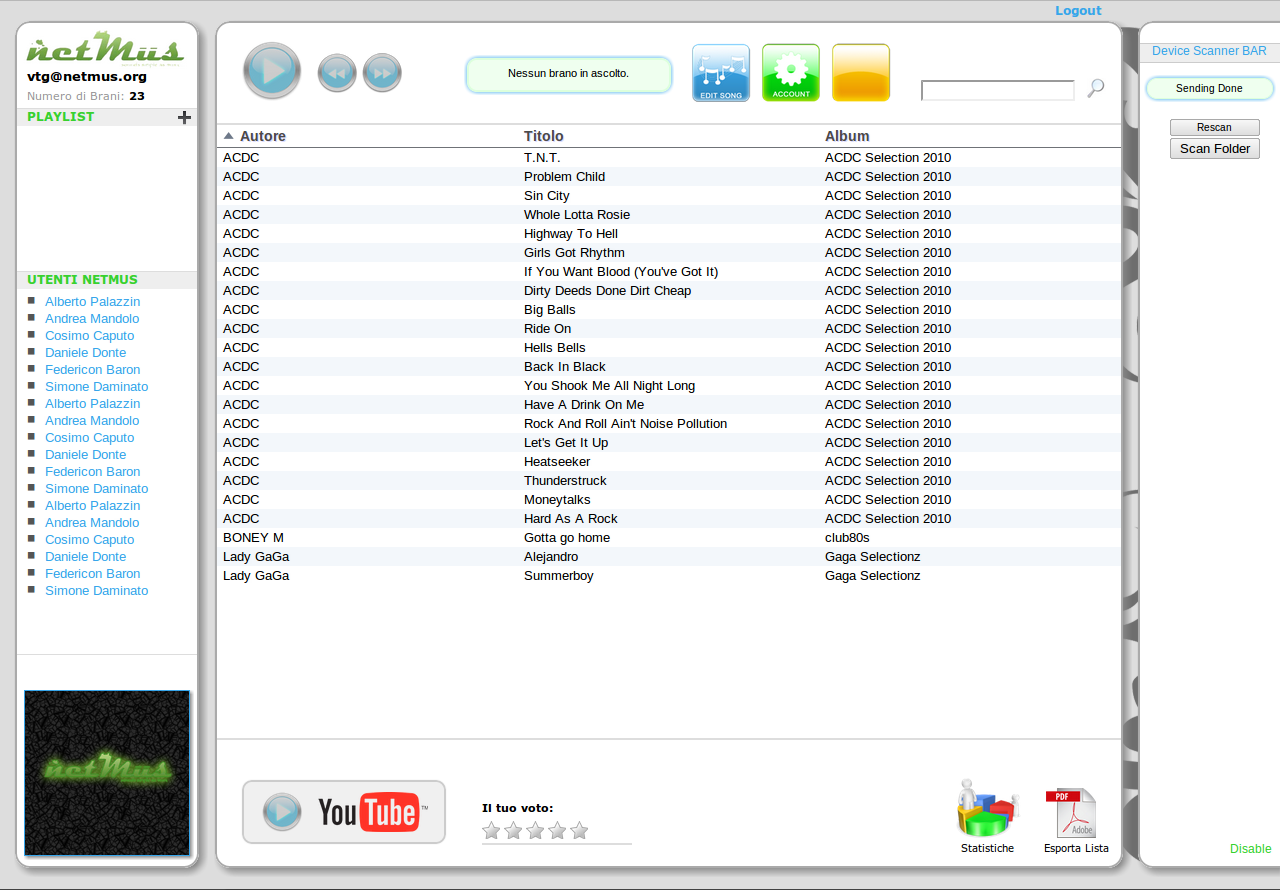
\includegraphics[width=15cm]{img/MU/song_loaded.png}
\caption{View with some songs on the Music Library}
\label{fig:fineUpload}
\end{figure}

Once the files have been sent, they appear inside your music library.
Now it's possible for you to start using \co{NetMus} functionalities.\\

All the actions that you can perform to take advantage of \co{NetMus} are listed
in subparagraphs some lines below for searching and viewing comfort.

\newpage
\section{Permitted Actions}
In the section below we present all the actions that you are allowed to perform
to take advantage of the product's functionalities.

\subsection{Display Modality}

The library is the central part of \co{NetMus}. Here you can find an ordinate
list of your songs saved by the scanning process of your devices. It's possible
to have two different views of the same library.\\
\\
The first is the list modality (figure \ref{fig:fineUpload}), that is the
default modality. In this way songs are listed with the informations about the title, the artist and the
album. You can also order your songs by clicking on the superior bar the voice
``artist'', ``title'', ``album''.\\

The second is the ``cover mode'' modality (figure
\ref{fig:coverMode}) in which your songs are listed with
the cover of their own album. This is a nicer way to view the songs, and it is also
a better way to recognized the same album's songs.\\

\begin{figure}[!htbp]
  \centering
  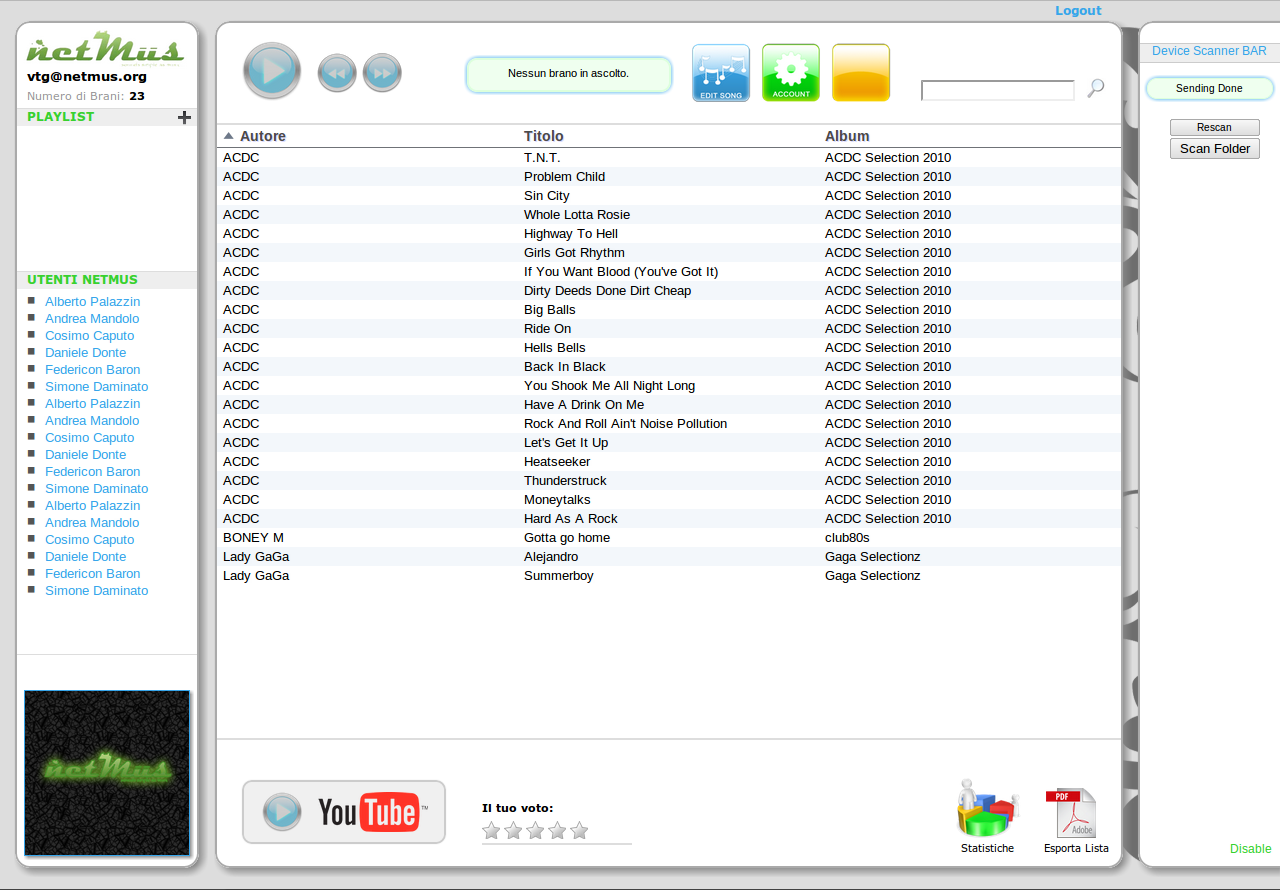
\includegraphics[width=14cm]{img/MU/song_loaded.png}
\caption{Interface with ``cover mode''}
\label{fig:coverMode}
\end{figure}

\subsection{Listening a song in streaming}

Let's look now at the most interesting function of the
product, the streaming.\\
If you want to listen one of your songs, you just have to select it from the
library, then click on play button of the top player, or the
bottom YouTube player (figure \ref{fig:play}).\\
\begin{figure}[!htbp]
  \centering
  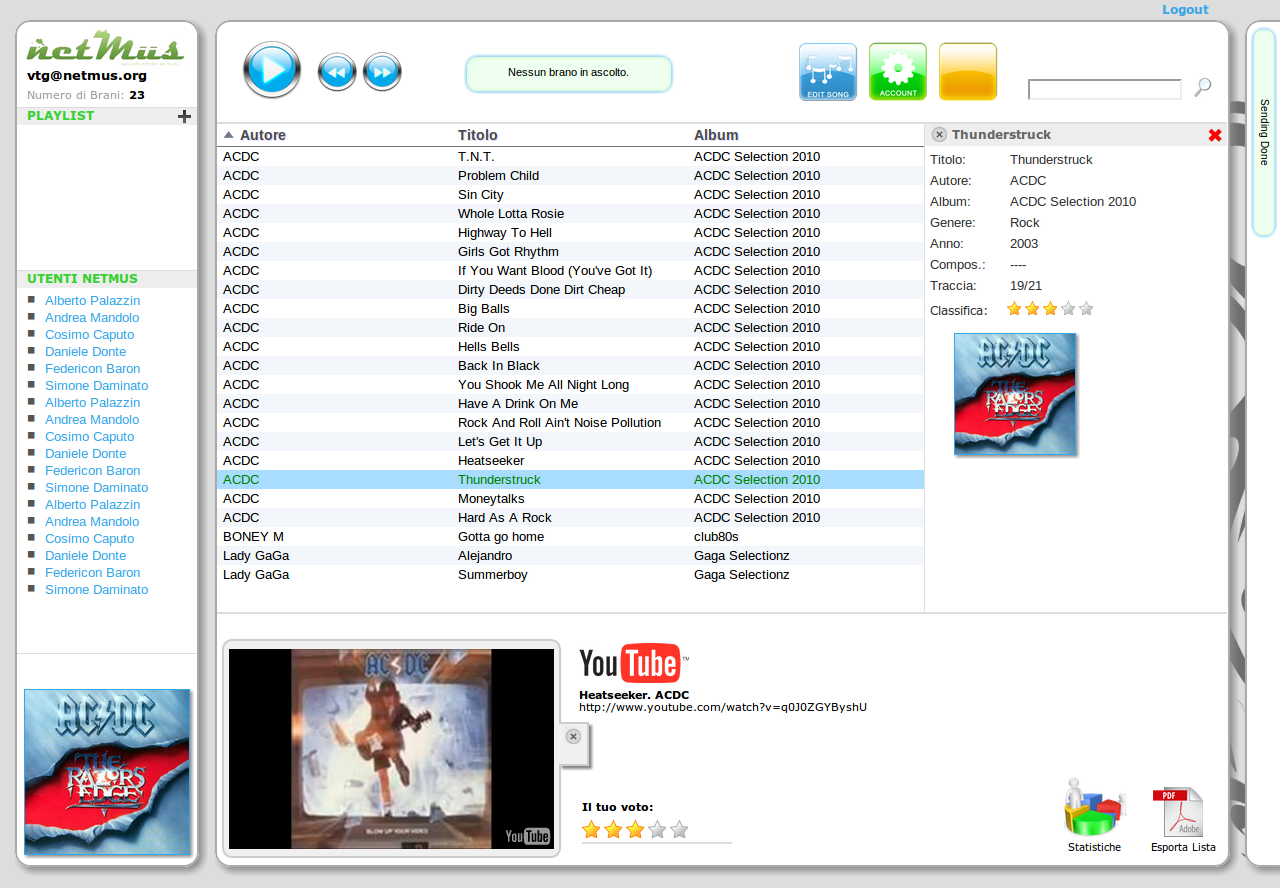
\includegraphics[width=15cm]{img/MU/player_youtube.png}
\caption{A video being reproduced with the YouTube player}
\label{fig:play}
\end{figure} 

The function of the two players is the same, but they have some differences.
The player at the top of the page (1) allows to play a song, but also
allows to shift at the next song or the previous, meanwhile the bottom player
transforms themselves in a YouTube streaming video player, where your selected song
is reproduced. Furthermore that player shows YouTube link to the video, and if
you click on it you will be redirected to the YouTube page of the song video.\\
It is possible to give a rank to the song (2) from 1 to 5, clicking on the right
star (look at \ref{cap:voto}).\\

To stop a song, you can pause using the button on the top player (1), or totally
close the streaming clicking on the ``x'' on the top right corner of the video
(3).\\

At the end of a song, the player will automatically play the next: if the song
was selected from the catalog, the next will be from there, but if the song was
initially selected from a playlist, it will play the next song of that
playlist.\\

\subsection{Create a Playlist}

Creating a \underline{playlist} is a very simple operation that allows you to
have an ordinate sequence of your favorite songs.\\
If you want to create a playlist (figure \ref{fig:playlist}) you just have to
click on the ``+'' button on the left menu near the voice ``PLAYLIST'' (1). It
will appear a field in which you can enter the title of the playlist. Once you insert the title you push
enter button and the playlist will be created (2).\\

\begin{figure}[!htbp]
  \centering
  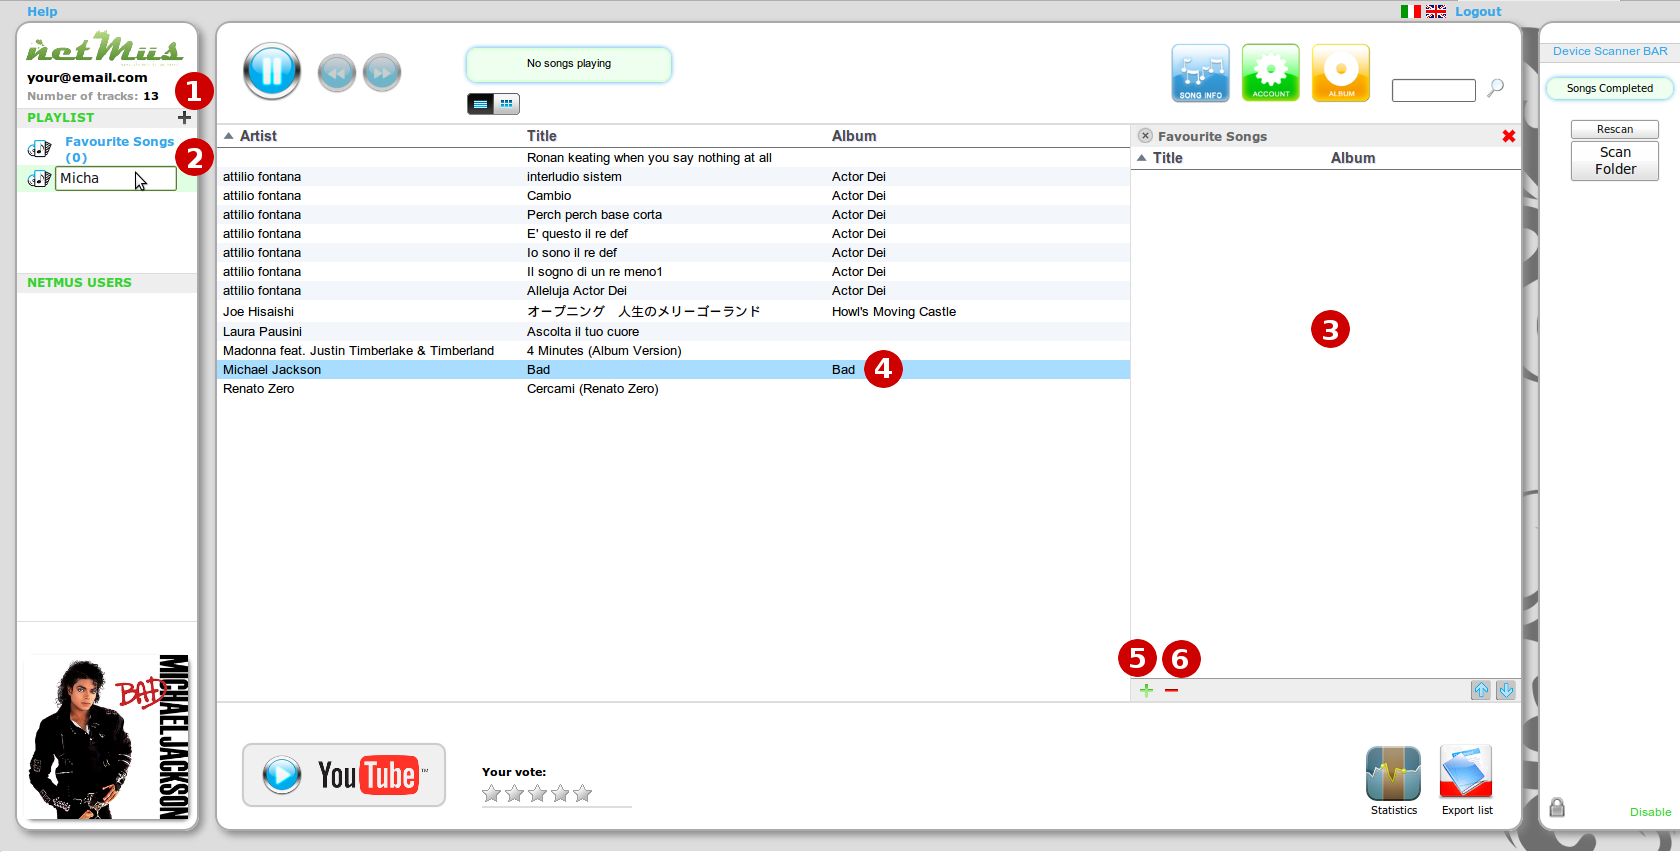
\includegraphics[width=15cm]{img/MU/new_playlist.png}
\caption{NetMus homepage with playlist menu}
\label{fig:playlist}
\end{figure}

Now you just need to insert songs that you want in your playlist. To do this
action you just have to click on the playlist name, it will appear a new window
(3), empty for the moment, in where you will find all playlist's songs. To
insert a new song in the playlist you have to select it (4) and double click on
it, or click on the ``+'' green button (5).\\ If you want to remove a song from
the playlist you have to select it from the frame of the playlist, and then click on the ``-''
red button (6), or press the ``Del'' button on the keyboard (somethimes also
called ``Canc'').\\

Finally if you want to delete a playlist you just have to click on the red ``X''
that is at the top-right side of the playlist details window.

\subsection{Songs Details}

If you want to view the complete informations about a song (figure
\ref{fig:dettagli}) you just have to
double click on it. It will appear a small window with a list of
all the informations of the song.\\
Note that this operation is not performed with a open playlist,
otherwise instead of displaying the information of the song, the song
will be added to the playlist.\\

\begin{figure}[!htbp]
  \centering
  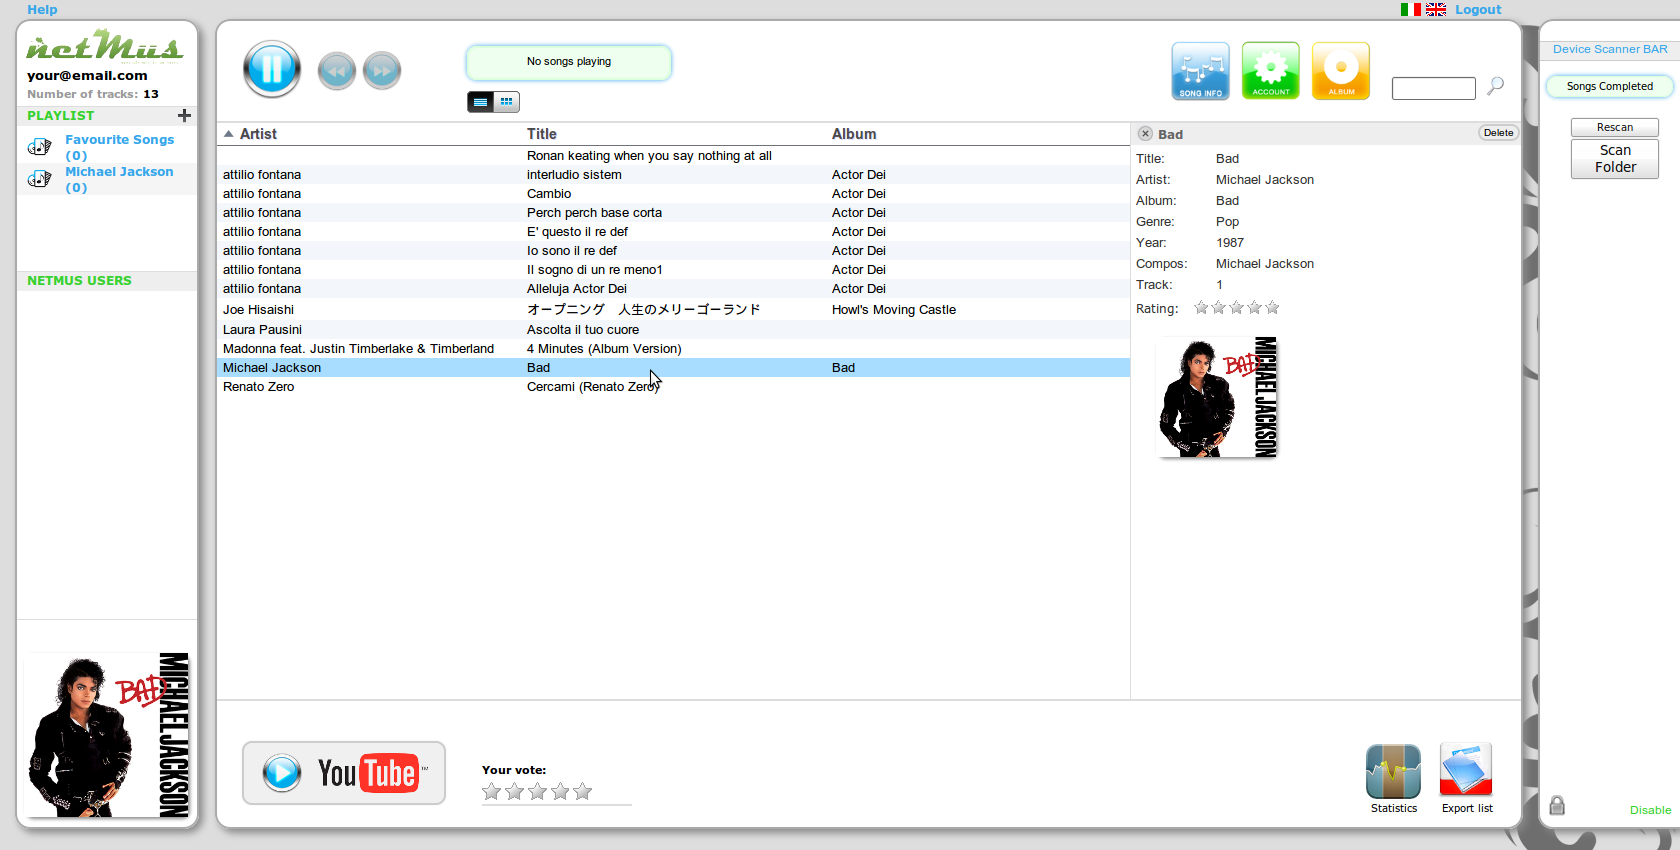
\includegraphics[width=15cm]{img/MU/info_song.png}
\caption{Song details}
\label{fig:dettagli}
\end{figure}

In the details you can see the song's title, author, album, genre, year,
composer, track number, evaluation and cover.\\
The evaluation is a functionality that will be explained better later.\\
The covers are searched and saved when the songs are sent to the library.

\subsection{Delete a song from your library}

To delete a song from your own library you just have to do a double click it, opening 
the details frame. Then on the details window that appeared you have to
click on the red ``Delete song'' button, and the song will be deleted from your
library.

\subsection{Searching a song on your library}

When you want to search a song in your library, you can use the right
\underline{form} (figure \ref{fig:appletbarAperta}, the element 4). This form is
placed on the top-right side of the page, and it allows to search a song on your
library only writing the title, album or artist's song. The searching process
is in real time, that means that all the results are shown in the center
library while you are typing.

\subsection{Modify your profile's informations (change password too)}

In the \co{NetMus} system it is possible to add new informations about your
profile.\\
You can perform this operation by clicking on the green button ``Account''. It
will appear a pop-up with a list of informations that you can complete (figure
\ref{fig:profilo}). These informations has to be inserted into those form.\\
\begin{figure}[!htbp]
  \centering
  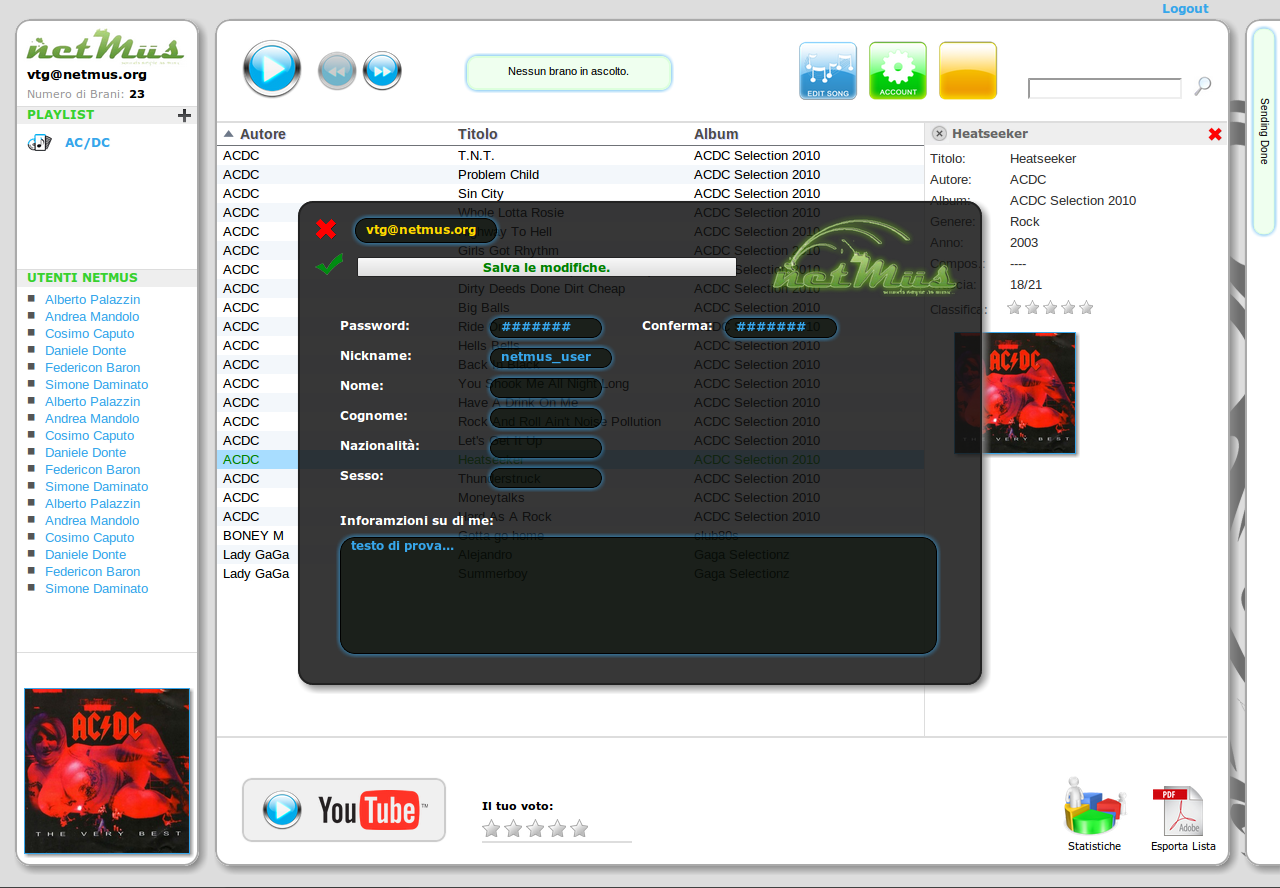
\includegraphics[width=15cm]{img/MU/profile_view.png}
\caption{View with the informations of the profile account}
\label{fig:profilo}
\end{figure}

You can add to your profile a complete nickname, name, surname, nationality, sex
and a small description about yourself. From this view it's also possible to change
your password.\\

In particular, to change the password, you must enter twice the new
password you will use in the appropriate fields (1). \\

When you have finished inserting all the informations you can click ``Save
changes'' (2), or click on the grey ``X'' (3) to abort the operation.\\

To delete your account instead, click on the red ``X'' (4): will be asked if you
really want to do this.

\subsection{Set rating for a song}
\label{cap:voto}
\co{NetMus} give you the possibility rate a song from one to five
stars.\\
Your rating will be added to all the ratings given by all the other users who
have the same song on their library and the average of all the votes will appear
in the details of the song.\\
To set a rating you have just to select the song from the library, then click on
the star number that you want at the bottom side of the page. The rating will be
automatically registered in the informations of this song.

\subsection{Creating a Google document of your music library}

This original function allows you to export your library to a Google document
that you can later print.\\
You just have to click on the bottom-right side on the button ``Export List''
to create your document. When you have clicked it, the system will automatically
generate a Google document and you will be able to view it: you can print it or
just save it on your PC.

\subsection{View system and your account's statistics}

To view statistics, simply click on the button
`` Statistics''in the lower right. Will then appear a pop-up with the
statistics relating to your account
(more played song, favorite genre, favorite author, etc. ..).

\newpage
\section{Errors and their Possible Reasons}

\subsection*{The USB device can't be scanned}
\begin{itemize}
  \item maybe the DEVICE SCANNER BAR isn't enable. Check on the DEVICE SCANNER
  BAR menu the label on the bottom-right side: the scanning process is disabled
  if the button displays the red word ``Enable''.
  \item if it had not been given permission to the applet to be executed, is
   normal it does not work. In this case, close the browser and
   reopen, returning to \co{NetMus} you will get asked again for permission.
\end{itemize}

\subsection*{Some songs that were in the device haven't been stored in the
library}
\begin{itemize}
  \item maybe these songs had been analysed some time before. To be sure of
  this, you can check the log that \co{NetMus} create inside your device with
  the list of the scanned songs.
  \item your mp3 songs hasn't all the most important tags complete. If an mp3
  file hasn't the tag artist, album and title complete with information, the
  song will not be stored on your library because it's impossible to identify
  what song is that.
  \item the song has tags, but they're corrupted. Sometimes can happen, especially
  with downloaded songs, that tags are present but they're not readable. Try to 
  modify them with any program and to save them, probably it will resolve this problem.
\end{itemize}

\subsection*{The song reproduced by the YouTube player is not the correct one}
\begin{itemize}
  \item unfortunately, research on YouTube is not always successful: this thing
   does not depend on our software.
  \item tags of the song you want are wrong and therefore
   search for that song produces erroneous results. Edit information
   of that song to solve the problem.
\end{itemize}

\subsection*{The album cover does not appear}
\begin{itemize}
  \item apparently the album cover in question wasn't
   found from our search service on the network. This is possible if
   the album isn't common, or if the tags of the
   song are wrong or badly written.
\end{itemize}

\listoffigures
\addcontentsline{toc}{chapter}{Index Figures}

\appendix % inizio appendice
\chapter{Most Common Error Messages}
\thispagestyle{fancy}

Here we present the error messages you may encounter using \co{NetMus}: for
convenience they are divided into sections, depending on the context in which
they may arise.
\section{Login/registration}
\begin{description}
	\item[Impossible to connect to database :] generic error that
	indicates an internal problem of the software. The software may be down for
	maintenance, try later.
	\item[Error: password must be at least 5 characters :] you can use the
	password you prefer, but there is a restriction: its lenght must be at least 5,
	so you have to choose a longer one.
	\item[Error: passwords do not match :] to confirm the
	chosen password it has to be repeated in the field, and this error appears
	when the two passwords do not match, usually indicates a typing error.
	\item[Error: invalid e-mail :] the inserted email isn't valid:
	a valid email is formatted like this: account@provider.domain (for example:
	andrew@google.com).
\end{description}

\section{AppletBar - adding new tracks}
\begin{description}
	\item [XML Error :] generic error that indicates a serious problem parsing mp3
	infos. Try to scan those songs again: if the problem persists, it means
	there are one or more tracks that create problems, you can try to make it
	analyze only a part of mp3s at a time.
	\item [Sending Error :] there is a communication problem with the applet:
	try to close and reopen the browser, returning to \co{NetMus}. If
	you still have the same error message, update the Java Virtual
	Machine.
	\item [Sending Error: problem with sending song to the server :] there is a
	communication problem with the server, try to restart \co{NetMus}.
\end{description}

\section{Playlist}
\begin{description}
	\item [Error: new playlist not created :] indicates that it was not possible
	to create a new playlist. Probably one already exists with the same name.
	\item [Error: playlist not removed :] it was not possible
	to remove the playlist: refresh the page.
	\item [Error: song not added to playlist :] it was not possible
	to add the song to that playlist: refresh the page.
	\item [Error: song not removed to playlist :] it was not possible
	to remove the song from the playlist: refresh the page.
	\item [Error: playlist not loaded :] There was an error loading the playlist, 
	probably due to a communication error with the server. Please retry to load it
	and possibly update the page if the problem persists, it is probably corrupt,
	then you should delete and recreate it.
	\item [Impossible to move the song :] there was a mistake to move a song in the
	playlist: reload it and try again.
\end{description}

\section{Profile}
\begin{description}
	\item[Error: profile not modified :] there was an error saving the latest
	changes to the profile. Try again.
	\item[Error: related user not found :] there was an error loading related
	users. However, this does not affect the functionality of the
	system: you can continue to use it normally, or update the page.
	\item[Error: profile not loaded :] serious error when loading the user profile.
	Try to restart your web browser.
	\item[Error: User Profile not deleted :] there was an error deleting the
	profile. Try again later.
\end{description}

\section{Songs}
\begin{description}
	\item[Error: song not removed :] there was an error removing the song.
	Refresh the page and try again.
	\item[Error: song info not loaded :] there was an error loading infos about a
	song. Refresh the page.
	\item[Error: rating not given :] have not been able to save the vote for that
	song: try again, and if necessary updated the page.
	\item[Error: statistics not updated :] statistics of the system is out of date:
	you can still use the system easily and safely ignoring this error message.
	\item[Error: document not generated :] was not possible to generate the
	document, most likely due to external services upon which supports this
	function: try again later.
	\item[No songs voted :] simply indicates that the user has not voted any song
	yet.
	\item[No songs has score :] simply indicates that users have not voted any song
	yet, then there isn't the most popular songs than others.
\end{description}

\chapter{Glossary}
\thispagestyle{fancy}

\subsection*{Web Browser:} program that allows any user to navigate through the
internet. Internet Explorer, NetScape and Firefox are web browsers. 
\subsection*{Cloud computing:} a group of computer technologies that allows to
take advantage of many resources allocate in remote. 
\subsection*{Directory:}
folder of your PC. 
\subsection*{Mass storage devices:} external hard disk, USB pens, Mp3 players
etc. 
\subsection*{Form:} part of the graphical inteface, where you can insert some
text. 
\subsection*{Nickname:} user's name.
\subsection*{Playlist:} a song list that you can create to listen all the songs
that you like more and in the order that you prefer. 
\subsection*{Social network:} online community, made by persons that have common interests
and/or activity.
\subsection*{Streaming:} is a multimedia service that allows to see video and
listen audio files from a remote source that sent all these informations to
many destinations through telecommunications network.

\end{document}